\documentclass{article}
%%%%%%%%%%%%%%%%%%%%%%%%%%%%%%%%%
% PACKAGE IMPORTS
%%%%%%%%%%%%%%%%%%%%%%%%%%%%%%%%%
\usepackage[framemethod=TikZ]{mdframed}
\usepackage{amsthm}
\usepackage{tikzsymbols}
\usepackage[tmargin=2.5cm,rmargin=2cm,lmargin=2.5cm,margin=0.85in,bmargin=2.5cm,footskip=.2in]{geometry}
\linespread{1.3}
\usepackage{amsmath,amsfonts,amsthm,amssymb,mathtools}
\usepackage[varbb]{newpxmath}
\usepackage{xfrac}
\usepackage[makeroom]{cancel}
\usepackage{bookmark}
\usepackage{enumitem}
\usepackage{hyperref,theoremref}
\hypersetup{
	pdftitle={Assignment},
	colorlinks=true, linkcolor=doc!90,
	bookmarksnumbered=true,
	bookmarksopen=true
}
\usepackage[most,many,breakable]{tcolorbox}
\usepackage{xcolor}
\usepackage{varwidth}
\usepackage{etoolbox}
\usepackage{nameref}
\usepackage{multicol,array}
\usepackage{tikz-cd}
\usepackage[ruled,vlined,linesnumbered]{algorithm2e}
\usepackage{comment} % enables the use of multi-line comments (\ifx \fi) 
\usepackage{import}
\usepackage{xifthen}
\usepackage{pdfpages}
\usepackage{transparent}
\usepackage[bottom]{footmisc}
\usepackage[utf8]{inputenc} % allow utf-8 input
\usepackage{braket}
\usepackage{wrapfig}			  %Kontekstom osjetljivo navođenje
\usepackage{csquotes}			  %Kontekstom osjetljivo navođenje
\usepackage{graphicx}       %Slike i slično
\usepackage[T1]{fontenc}    % use 8-bit T1 fonts
\usepackage{url}            % simple URL typesetting
\usepackage{booktabs}       % professional-quality tables
\usepackage{nicefrac}       % compact symbols for 1/2, etc.
\usepackage{float}
\usepackage{caption}
\usepackage{subcaption}
\usepackage{listings}
\usepackage[english,croatian]{babel}
\usepackage{titlesec}				%Za naslovnu stranicu

\counterwithin{figure}{section}
\urlstyle{same}
\numberwithin{equation}{section}
\hyphenation{pergamon} % riječ u argumentu (pergamon) se ne rastavlja s crticom; ne smije imat specijalna slova. č. ž... - rastavljam ju naredbom \- (npr. išče\-zava)
\setlength\parindent{0pt} % u novom paragrafu: indent=0
\setlength{\parskip}{10pt} % postavlja željeni vertikalni razmak između paragrafa
\setlength{\skip\footins}{2cm} % razmak između glavnog teksta i fusnota
\renewcommand{\thefootnote}{$\ddagger$} % želim dagger za oznaku fusnota
\newcommand{\HRule}{\rule{\linewidth}{0.4mm}} % nova naredba za horizontalne linije na naslovnoj stranici
\newlength{\mylen}
\setcounter{secnumdepth}{4}
\titleformat{\paragraph}
{\normalfont\normalsize\bfseries}{\theparagraph}{1em}{}


%%%%%%%%%%%%%%%%%%%%%%%%%%%%%%%%%%%%%%%%%%%
% TABLE OF CONTENTS
%%%%%%%%%%%%%%%%%%%%%%%%%%%%%%%%%%%%%%%%%%%

\usepackage{tikz}
\definecolor{doc}{RGB}{0,60,110}
\usepackage{titletoc}
\contentsmargin{0cm}
\titlecontents{chapter}[3.7pc]
{\addvspace{30pt}%
	\begin{tikzpicture}[remember picture, overlay]%
		\draw[fill=doc!60,draw=doc!60] (-7,-.1) rectangle (-0.9,.5);%
		\pgftext[left,x=-3.5cm,y=0.2cm]{\color{white}\Large\sc\bfseries Chapter\ \thecontentslabel};%
	\end{tikzpicture}\color{doc!60}\large\sc\bfseries}%
{}
{}
{\;\titlerule\;\large\sc\bfseries Page \thecontentspage
	\begin{tikzpicture}[remember picture, overlay]
		\draw[fill=doc!60,draw=doc!60] (2pt,0) rectangle (4,0.1pt);
	\end{tikzpicture}}%
\titlecontents{section}[3.7pc]
{\addvspace{2pt}}
{\contentslabel[\thecontentslabel]{2pc}}
{}
{\hfill\small \thecontentspage}
[]
\titlecontents*{subsection}[3.7pc]
{\addvspace{-1pt}\small}
{}
{}
{\ --- \small\thecontentspage}
[ \textbullet\ ][]

\makeatletter
\renewcommand{\tableofcontents}{%
	\chapter{%
	  \vspace{-20\p@}%
	  \begin{tikzpicture}[remember picture, overlay]%
		  \pgftext[right,x=15cm,y=0.2cm]{\color{doc!60}\Huge\sc\bfseries \contentsname};%
		  \draw[fill=doc!60,draw=doc!60] (13,-.75) rectangle (20,1);%
		  \clip (13,-.75) rectangle (20,1);
		  \pgftext[right,x=15cm,y=0.2cm]{\color{white}\Huge\sc\bfseries \contentsname};%
	  \end{tikzpicture}}%
	\@starttoc{toc}}
\makeatother


%%%%%%%%%%%%
%% KUTIJE %%
%%%%%%%%%%%%
%%%%%%%%%%%%%%%%%%%%%%%%%%%%%%
%Theorem
\newcounter{teorem}[section] \setcounter{teorem}{0}
\renewcommand{\theteorem}{\arabic{section}.\arabic{teorem}}
\newenvironment{teorem}[2][]{%
	\refstepcounter{teorem}%
	\ifstrempty{#1}%
	{\mdfsetup{%
			frametitle={%
					\tikz[baseline=(current bounding box.east),outer sep=0pt]
					\node[anchor=east,rectangle,fill=blue!20]
					{\strut Teorem~\thetheo};}}
	}%
	{\mdfsetup{%
			frametitle={%
					\tikz[baseline=(current bounding box.east),outer sep=0pt]
					\node[anchor=east,rectangle,fill=blue!20]
					{\strut Teorem~\thetheo:~#1};}}%
	}%
	\mdfsetup{innertopmargin=10pt,linecolor=blue!20,%
		linewidth=2pt,topline=true,%
		frametitleaboveskip=\dimexpr-\ht\strutbox\relax
	}
	\begin{mdframed}[]\relax%
		\label{#2}}{\end{mdframed}}
%%%%%%%%%%%%%%%%%%%%%%%%%%%%%%
%Proof
\newcounter{dokaz}[section]\setcounter{dokaz}{0}
\renewcommand{\thedokaz}{\arabic{section}.\arabic{dokaz}}
\newenvironment{dokaz}[2][]{%
	\refstepcounter{dokaz}%
	\ifstrempty{#1}%
	{\mdfsetup{%
			frametitle={%
					\tikz[baseline=(current bounding box.east),outer sep=0pt]
					\node[anchor=east,rectangle,fill=red!20]
					{\strut Dokaz~\theprf};}}
	}%
	{\mdfsetup{%
			frametitle={%
					\tikz[baseline=(current bounding box.east),outer sep=0pt]
					\node[anchor=east,rectangle,fill=red!20]
					{\strut Dokaz~\theprf:~#1};}}%
	}%
	\mdfsetup{innertopmargin=10pt,linecolor=red!20,%
		linewidth=2pt,topline=true,%
		frametitleaboveskip=\dimexpr-\ht\strutbox\relax
	}
	\begin{mdframed}[]\relax%
		\label{#2}}{\qed\end{mdframed}}
%%%%%%%%%%%%%%%%%%%%%%%%%%%%%%

\newcommand{\eps}{\epsilon}
\newcommand{\veps}{\varepsilon}
\newcommand{\ol}{\overline}
\newcommand{\ul}{\underline}
\newcommand{\wt}{\widetilde}
\newcommand{\wh}{\widehat}
\newcommand{\vocab}[1]{\textbf{\color{blue} #1}}
\providecommand{\half}{\frac{1}{2}}
\newcommand{\dang}{\measuredangle} %% Directed angle
\newcommand{\ray}[1]{\overrightarrow{#1}}
\newcommand{\seg}[1]{\overline{#1}}
\newcommand{\arc}[1]{\wideparen{#1}}
\DeclareMathOperator{\cis}{cis}
\DeclareMathOperator*{\lcm}{lcm}
\DeclareMathOperator*{\argmin}{arg min}
\DeclareMathOperator*{\argmax}{arg max}
\newcommand{\cycsum}{\sum_{\mathrm{cyc}}}
\newcommand{\symsum}{\sum_{\mathrm{sym}}}
\newcommand{\cycprod}{\prod_{\mathrm{cyc}}}
\newcommand{\symprod}{\prod_{\mathrm{sym}}}
\newcommand{\Qed}{\begin{flushright}\qed\end{flushright}}
\newcommand{\parinn}{\setlength{\parindent}{1cm}}
\newcommand{\parinf}{\setlength{\parindent}{0cm}}
% \newcommand{\norm}{\|\cdot\|}
\newcommand{\inorm}{\norm_{\infty}}
\newcommand{\opensets}{\{V_{\alpha}\}_{\alpha\in I}}
\newcommand{\oset}{V_{\alpha}}
\newcommand{\opset}[1]{V_{\alpha_{#1}}}
\newcommand{\lub}{\text{lub}}
\newcommand{\del}[2]{\frac{\partial #1}{\partial #2}}
\newcommand{\Del}[3]{\frac{\partial^{#1} #2}{\partial^{#1} #3}}
\newcommand{\deld}[2]{\dfrac{\partial #1}{\partial #2}}
\newcommand{\Deld}[3]{\dfrac{\partial^{#1} #2}{\partial^{#1} #3}}
\newcommand{\lm}{\lambda}
\newcommand{\uin}{\mathbin{\rotatebox[origin=c]{90}{$\in$}}}
\newcommand{\usubset}{\mathbin{\rotatebox[origin=c]{90}{$\subset$}}}
\newcommand{\lt}{\left}
\newcommand{\rt}{\right}
\newcommand{\bs}[1]{\boldsymbol{#1}}
\newcommand{\exs}{\exists}
\newcommand{\st}{\strut}
\newcommand{\dps}[1]{\displaystyle{#1}}

\newcommand{\sol}{\setlength{\parindent}{0cm}\textbf{\textit{Solution:}}\setlength{\parindent}{1cm} }
\newcommand{\solve}[1]{\setlength{\parindent}{0cm}\textbf{\textit{Solution: }}\setlength{\parindent}{1cm}#1 \Qed}

%From M275 "Topology" at SJSU
\newcommand{\id}{\mathrm{id}}
\newcommand{\taking}[1]{\xrightarrow{#1}}
\newcommand{\inv}{^{-1}}

%From M170 "Introduction to Graph Theory" at SJSU
\DeclareMathOperator{\diam}{diam}
\DeclareMathOperator{\ord}{ord}
\newcommand{\defeq}{\overset{\mathrm{def}}{=}}

%From the USAMO .tex files
\newcommand{\ts}{\textsuperscript}
\newcommand{\dg}{^\circ}
\newcommand{\ii}{\item}

% % From Math 55 and Math 145 at Harvard
% \newenvironment{subproof}[1][Proof]{%
% \begin{proof}[#1] \renewcommand{\qedsymbol}{$\blacksquare$}}%
% {\end{proof}}

\newcommand{\liff}{\leftrightarrow}
\newcommand{\lthen}{\rightarrow}
\newcommand{\opname}{\operatorname}
\newcommand{\surjto}{\twoheadrightarrow}
\newcommand{\injto}{\hookrightarrow}
\newcommand{\On}{\mathrm{On}} % ordinals
\DeclareMathOperator{\img}{im} % Image
\DeclareMathOperator{\Img}{Im} % Image
\DeclareMathOperator{\coker}{coker} % Cokernel
\DeclareMathOperator{\Coker}{Coker} % Cokernel
\DeclareMathOperator{\Ker}{Ker} % Kernel
\DeclareMathOperator{\rank}{rank}
\DeclareMathOperator{\Spec}{Spec} % spectrum
\DeclareMathOperator{\Tr}{Tr} % trace
\DeclareMathOperator{\pr}{pr} % projection
\DeclareMathOperator{\ext}{ext} % extension
\DeclareMathOperator{\pred}{pred} % predecessor
\DeclareMathOperator{\dom}{dom} % domain
\DeclareMathOperator{\ran}{ran} % range
\DeclareMathOperator{\Hom}{Hom} % homomorphism
\DeclareMathOperator{\Mor}{Mor} % morphisms
\DeclareMathOperator{\End}{End} % endomorphism

% Things Lie
\newcommand{\kb}{\mathfrak b}
\newcommand{\kg}{\mathfrak g}
\newcommand{\kh}{\mathfrak h}
\newcommand{\kn}{\mathfrak n}
\newcommand{\ku}{\mathfrak u}
\newcommand{\kz}{\mathfrak z}
\DeclareMathOperator{\Ext}{Ext} % Ext functor
\DeclareMathOperator{\Tor}{Tor} % Tor functor
\newcommand{\gl}{\opname{\mathfrak{gl}}} % frak gl group
\renewcommand{\sl}{\opname{\mathfrak{sl}}} % frak sl group chktex 6

% More script letters etc.
\newcommand{\SA}{\mathcal A}
\newcommand{\SB}{\mathcal B}
\newcommand{\SC}{\mathcal C}
\newcommand{\SF}{\mathcal F}
\newcommand{\SG}{\mathcal G}
\newcommand{\SH}{\mathcal H}
\newcommand{\OO}{\mathcal O}

\newcommand{\SCA}{\mathscr A}
\newcommand{\SCB}{\mathscr B}
\newcommand{\SCC}{\mathscr C}
\newcommand{\SCD}{\mathscr D}
\newcommand{\SCE}{\mathscr E}
\newcommand{\SCF}{\mathscr F}
\newcommand{\SCG}{\mathscr G}
\newcommand{\SCH}{\mathscr H}

% Mathfrak primes
\newcommand{\km}{\mathfrak m}
\newcommand{\kp}{\mathfrak p}
\newcommand{\kq}{\mathfrak q}

% number sets
\newcommand{\RR}[1][]{\ensuremath{\ifstrempty{#1}{\mathbb{R}}{\mathbb{R}^{#1}}}}
\newcommand{\NN}[1][]{\ensuremath{\ifstrempty{#1}{\mathbb{N}}{\mathbb{N}^{#1}}}}
\newcommand{\ZZ}[1][]{\ensuremath{\ifstrempty{#1}{\mathbb{Z}}{\mathbb{Z}^{#1}}}}
\newcommand{\QQ}[1][]{\ensuremath{\ifstrempty{#1}{\mathbb{Q}}{\mathbb{Q}^{#1}}}}
\newcommand{\CC}[1][]{\ensuremath{\ifstrempty{#1}{\mathbb{C}}{\mathbb{C}^{#1}}}}
\newcommand{\PP}[1][]{\ensuremath{\ifstrempty{#1}{\mathbb{P}}{\mathbb{P}^{#1}}}}
\newcommand{\HH}[1][]{\ensuremath{\ifstrempty{#1}{\mathbb{H}}{\mathbb{H}^{#1}}}}
\newcommand{\FF}[1][]{\ensuremath{\ifstrempty{#1}{\mathbb{F}}{\mathbb{F}^{#1}}}}
% expected value
\newcommand{\EE}{\ensuremath{\mathbb{E}}}
\newcommand{\charin}{\text{ char }}
\DeclareMathOperator{\sign}{sign}
\DeclareMathOperator{\Aut}{Aut}
\DeclareMathOperator{\Inn}{Inn}
\DeclareMathOperator{\Syl}{Syl}
\DeclareMathOperator{\Gal}{Gal}
\DeclareMathOperator{\GL}{GL} % General linear group
\DeclareMathOperator{\SL}{SL} % Special linear group

%---------------------------------------
% BlackBoard Math Fonts :-
%---------------------------------------

%Captital Letters
\newcommand{\bbA}{\mathbb{A}}	\newcommand{\bbB}{\mathbb{B}}
\newcommand{\bbC}{\mathbb{C}}	\newcommand{\bbD}{\mathbb{D}}
\newcommand{\bbE}{\mathbb{E}}	\newcommand{\bbF}{\mathbb{F}}
\newcommand{\bbG}{\mathbb{G}}	\newcommand{\bbH}{\mathbb{H}}
\newcommand{\bbI}{\mathbb{I}}	\newcommand{\bbJ}{\mathbb{J}}
\newcommand{\bbK}{\mathbb{K}}	\newcommand{\bbL}{\mathbb{L}}
\newcommand{\bbM}{\mathbb{M}}	\newcommand{\bbN}{\mathbb{N}}
\newcommand{\bbO}{\mathbb{O}}	\newcommand{\bbP}{\mathbb{P}}
\newcommand{\bbQ}{\mathbb{Q}}	\newcommand{\bbR}{\mathbb{R}}
\newcommand{\bbS}{\mathbb{S}}	\newcommand{\bbT}{\mathbb{T}}
\newcommand{\bbU}{\mathbb{U}}	\newcommand{\bbV}{\mathbb{V}}
\newcommand{\bbW}{\mathbb{W}}	\newcommand{\bbX}{\mathbb{X}}
\newcommand{\bbY}{\mathbb{Y}}	\newcommand{\bbZ}{\mathbb{Z}}

%---------------------------------------
% MathCal Fonts :-
%---------------------------------------

%Captital Letters
\newcommand{\mcA}{\mathcal{A}}	\newcommand{\mcB}{\mathcal{B}}
\newcommand{\mcC}{\mathcal{C}}	\newcommand{\mcD}{\mathcal{D}}
\newcommand{\mcE}{\mathcal{E}}	\newcommand{\mcF}{\mathcal{F}}
\newcommand{\mcG}{\mathcal{G}}	\newcommand{\mcH}{\mathcal{H}}
\newcommand{\mcI}{\mathcal{I}}	\newcommand{\mcJ}{\mathcal{J}}
\newcommand{\mcK}{\mathcal{K}}	\newcommand{\mcL}{\mathcal{L}}
\newcommand{\mcM}{\mathcal{M}}	\newcommand{\mcN}{\mathcal{N}}
\newcommand{\mcO}{\mathcal{O}}	\newcommand{\mcP}{\mathcal{P}}
\newcommand{\mcQ}{\mathcal{Q}}	\newcommand{\mcR}{\mathcal{R}}
\newcommand{\mcS}{\mathcal{S}}	\newcommand{\mcT}{\mathcal{T}}
\newcommand{\mcU}{\mathcal{U}}	\newcommand{\mcV}{\mathcal{V}}
\newcommand{\mcW}{\mathcal{W}}	\newcommand{\mcX}{\mathcal{X}}
\newcommand{\mcY}{\mathcal{Y}}	\newcommand{\mcZ}{\mathcal{Z}}



%---------------------------------------
% Bold Math Fonts :-
%---------------------------------------

%Captital Letters
\newcommand{\bmA}{\boldsymbol{A}}	\newcommand{\bmB}{\boldsymbol{B}}
\newcommand{\bmC}{\boldsymbol{C}}	\newcommand{\bmD}{\boldsymbol{D}}
\newcommand{\bmE}{\boldsymbol{E}}	\newcommand{\bmF}{\boldsymbol{F}}
\newcommand{\bmG}{\boldsymbol{G}}	\newcommand{\bmH}{\boldsymbol{H}}
\newcommand{\bmI}{\boldsymbol{I}}	\newcommand{\bmJ}{\boldsymbol{J}}
\newcommand{\bmK}{\boldsymbol{K}}	\newcommand{\bmL}{\boldsymbol{L}}
\newcommand{\bmM}{\boldsymbol{M}}	\newcommand{\bmN}{\boldsymbol{N}}
\newcommand{\bmO}{\boldsymbol{O}}	\newcommand{\bmP}{\boldsymbol{P}}
\newcommand{\bmQ}{\boldsymbol{Q}}	\newcommand{\bmR}{\boldsymbol{R}}
\newcommand{\bmS}{\boldsymbol{S}}	\newcommand{\bmT}{\boldsymbol{T}}
\newcommand{\bmU}{\boldsymbol{U}}	\newcommand{\bmV}{\boldsymbol{V}}
\newcommand{\bmW}{\boldsymbol{W}}	\newcommand{\bmX}{\boldsymbol{X}}
\newcommand{\bmY}{\boldsymbol{Y}}	\newcommand{\bmZ}{\boldsymbol{Z}}
%Small Letters
\newcommand{\bma}{\boldsymbol{a}}	\newcommand{\bmb}{\boldsymbol{b}}
\newcommand{\bmc}{\boldsymbol{c}}	\newcommand{\bmd}{\boldsymbol{d}}
\newcommand{\bme}{\boldsymbol{e}}	\newcommand{\bmf}{\boldsymbol{f}}
\newcommand{\bmg}{\boldsymbol{g}}	\newcommand{\bmh}{\boldsymbol{h}}
\newcommand{\bmi}{\boldsymbol{i}}	\newcommand{\bmj}{\boldsymbol{j}}
\newcommand{\bmk}{\boldsymbol{k}}	\newcommand{\bml}{\boldsymbol{l}}
\newcommand{\bmm}{\boldsymbol{m}}	\newcommand{\bmn}{\boldsymbol{n}}
\newcommand{\bmo}{\boldsymbol{o}}	\newcommand{\bmp}{\boldsymbol{p}}
\newcommand{\bmq}{\boldsymbol{q}}	\newcommand{\bmr}{\boldsymbol{r}}
\newcommand{\bms}{\boldsymbol{s}}	\newcommand{\bmt}{\boldsymbol{t}}
\newcommand{\bmu}{\boldsymbol{u}}	\newcommand{\bmv}{\boldsymbol{v}}
\newcommand{\bmw}{\boldsymbol{w}}	\newcommand{\bmx}{\boldsymbol{x}}
\newcommand{\bmy}{\boldsymbol{y}}	\newcommand{\bmz}{\boldsymbol{z}}

%---------------------------------------
% Scr Math Fonts :-
%---------------------------------------

\newcommand{\sA}{{\mathscr{A}}}   \newcommand{\sB}{{\mathscr{B}}}
\newcommand{\sC}{{\mathscr{C}}}   \newcommand{\sD}{{\mathscr{D}}}
\newcommand{\sE}{{\mathscr{E}}}   \newcommand{\sF}{{\mathscr{F}}}
\newcommand{\sG}{{\mathscr{G}}}   \newcommand{\sH}{{\mathscr{H}}}
\newcommand{\sI}{{\mathscr{I}}}   \newcommand{\sJ}{{\mathscr{J}}}
\newcommand{\sK}{{\mathscr{K}}}   \newcommand{\sL}{{\mathscr{L}}}
\newcommand{\sM}{{\mathscr{M}}}   \newcommand{\sN}{{\mathscr{N}}}
\newcommand{\sO}{{\mathscr{O}}}   \newcommand{\sP}{{\mathscr{P}}}
\newcommand{\sQ}{{\mathscr{Q}}}   \newcommand{\sR}{{\mathscr{R}}}
\newcommand{\sS}{{\mathscr{S}}}   \newcommand{\sT}{{\mathscr{T}}}
\newcommand{\sU}{{\mathscr{U}}}   \newcommand{\sV}{{\mathscr{V}}}
\newcommand{\sW}{{\mathscr{W}}}   \newcommand{\sX}{{\mathscr{X}}}
\newcommand{\sY}{{\mathscr{Y}}}   \newcommand{\sZ}{{\mathscr{Z}}}


%---------------------------------------
% Math Fraktur Font
%---------------------------------------

%Captital Letters
\newcommand{\mfA}{\mathfrak{A}}	\newcommand{\mfB}{\mathfrak{B}}
\newcommand{\mfC}{\mathfrak{C}}	\newcommand{\mfD}{\mathfrak{D}}
\newcommand{\mfE}{\mathfrak{E}}	\newcommand{\mfF}{\mathfrak{F}}
\newcommand{\mfG}{\mathfrak{G}}	\newcommand{\mfH}{\mathfrak{H}}
\newcommand{\mfI}{\mathfrak{I}}	\newcommand{\mfJ}{\mathfrak{J}}
\newcommand{\mfK}{\mathfrak{K}}	\newcommand{\mfL}{\mathfrak{L}}
\newcommand{\mfM}{\mathfrak{M}}	\newcommand{\mfN}{\mathfrak{N}}
\newcommand{\mfO}{\mathfrak{O}}	\newcommand{\mfP}{\mathfrak{P}}
\newcommand{\mfQ}{\mathfrak{Q}}	\newcommand{\mfR}{\mathfrak{R}}
\newcommand{\mfS}{\mathfrak{S}}	\newcommand{\mfT}{\mathfrak{T}}
\newcommand{\mfU}{\mathfrak{U}}	\newcommand{\mfV}{\mathfrak{V}}
\newcommand{\mfW}{\mathfrak{W}}	\newcommand{\mfX}{\mathfrak{X}}
\newcommand{\mfY}{\mathfrak{Y}}	\newcommand{\mfZ}{\mathfrak{Z}}
%Small Letters
\newcommand{\mfa}{\mathfrak{a}}	\newcommand{\mfb}{\mathfrak{b}}
\newcommand{\mfc}{\mathfrak{c}}	\newcommand{\mfd}{\mathfrak{d}}
\newcommand{\mfe}{\mathfrak{e}}	\newcommand{\mff}{\mathfrak{f}}
\newcommand{\mfg}{\mathfrak{g}}	\newcommand{\mfh}{\mathfrak{h}}
\newcommand{\mfi}{\mathfrak{i}}	\newcommand{\mfj}{\mathfrak{j}}
\newcommand{\mfk}{\mathfrak{k}}	\newcommand{\mfl}{\mathfrak{l}}
\newcommand{\mfm}{\mathfrak{m}}	\newcommand{\mfn}{\mathfrak{n}}
\newcommand{\mfo}{\mathfrak{o}}	\newcommand{\mfp}{\mathfrak{p}}
\newcommand{\mfq}{\mathfrak{q}}	\newcommand{\mfr}{\mathfrak{r}}
\newcommand{\mfs}{\mathfrak{s}}	\newcommand{\mft}{\mathfrak{t}}
\newcommand{\mfu}{\mathfrak{u}}	\newcommand{\mfv}{\mathfrak{v}}
\newcommand{\mfw}{\mathfrak{w}}	\newcommand{\mfx}{\mathfrak{x}}
\newcommand{\mfy}{\mathfrak{y}}	\newcommand{\mfz}{\mathfrak{z}}


% Customizing title
\renewcommand{\maketitlehooka}{\centering}
\renewcommand{\maketitlehookb}{\vspace{-1.5em}}

% Customizing abstract
\renewcommand{\abstractnamefont}{\normalfont\large\bfseries}
\renewcommand{\abstracttextfont}{\normalfont\normalsize}
\graphicspath{{./Images/}} % Where to take images from
%%%%%%%%%%%%%%%%%%%%%%%%%% Define some useful colors %%%%%%%%%%%%%%%%%%%%%%%%%%
\definecolor{ocre}{RGB}{243,102,25}
\definecolor{mygray}{RGB}{243,243,244}
\definecolor{deepGreen}{RGB}{26,111,0}
\definecolor{shallowGreen}{RGB}{235,255,255}
\definecolor{deepBlue}{RGB}{61,124,222}
\definecolor{shallowBlue}{RGB}{235,249,255}
%%%%%%%%%%%%%%%%%%%%%%%%%%%%%%%%%%%%%%%%%%%%%%%%%%%%%%%%%%%%%%%%%%%%%%%%%%%%%%%

%%%%%%%%%%%%%%%%%%%%%%%%%% Define an orangebox command %%%%%%%%%%%%%%%%%%%%%%%%
\newcommand\orangebox[1]{\fcolorbox{ocre}{mygray}{\hspace{1em}#1\hspace{1em}}}
%%%%%%%%%%%%%%%%%%%%%%%%%%%%%%%%%%%%%%%%%%%%%%%%%%%%%%%%%%%%%%%%%%%%%%%%%%%%%%%

%%%%%%%%%%%%%%%%%%%%%%%%%%%% English Environments %%%%%%%%%%%%%%%%%%%%%%%%%%%%%
\newtheoremstyle{mytheoremstyle}{3pt}{3pt}{\normalfont}{0cm}{\rmfamily\bfseries}{}{1em}{{\color{black}\thmname{#1}~\thmnumber{#2}}\thmnote{\,--\,#3}}
\newtheoremstyle{myproblemstyle}{3pt}{3pt}{\normalfont}{0cm}{\rmfamily\bfseries}{}{1em}{{\color{black}\thmname{#1}~\thmnumber{#2}}\thmnote{\,--\,#3}}
\theoremstyle{mytheoremstyle}
\newmdtheoremenv[linewidth=1pt,backgroundcolor=shallowGreen,linecolor=deepGreen,leftmargin=0pt,innerleftmargin=20pt,innerrightmargin=20pt,]{theorem}{Theorem}[section]
\theoremstyle{mytheoremstyle}
\newmdtheoremenv[linewidth=1pt,backgroundcolor=shallowBlue,linecolor=deepBlue,leftmargin=0pt,innerleftmargin=20pt,innerrightmargin=20pt,]{definition}{Definition}[section]
\theoremstyle{myproblemstyle}
\newmdtheoremenv[linecolor=black,leftmargin=0pt,innerleftmargin=10pt,innerrightmargin=10pt,]{problem}{Problem}[section]
%%%%%%%%%%%%%%%%%%%%%%%%%%%%%%%%%%%%%%%%%%%%%%%%%%%%%%%%%%%%%%%%%%%%%%%%%%%%%%%
\begin{document}
%%%%%%%%%%%%%%%%%%%%%%%%%%%%%%% Title & Author %%%%%%%%%%%%%%%%%%%%%%%%%%%%%%%%
\begin{titlepage}
	\begin{center}
		{\LARGE Univerza \textit{v Ljubljani}} \\[0.1cm]
		{\LARGE Fakulteta za \textit{matematiko in fiziko}} \\[1cm]
		\begin{figure}[h]
			\centering
			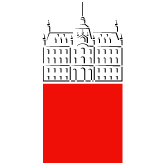
\includegraphics[width=0.25\textwidth]{UL logo.png}
			\label{fig:UL logo}
		\end{figure}
		{\large \textbf{Adrian Udovičić, mag. phys.}}\\[0.1cm]
		{\sc DISPOZICIJA DOKTORSKE DISERTACIJE}\\
		\vspace{1cm}

		{\bf \Large Ustvarjanje in teleportiranje prepletenosti za kvantna omrežja}\\
		\vspace{1cm}

		{\bf \Large Generating and teleporting entanglement for quantum networks}\\


		\vspace{3cm}

		{\large ADVISER: Rainer O. Kaltenbaek, assoc. prof. dr.\\

		\vspace{2cm}
		Znanstveno področje: Fizika\\
		\vspace{1cm}
		Ljubljana, 2025\date{}}
	\end{center}
\end{titlepage}
%%%%%%%%%%%%%%%%%%%%%%%%%%%%%%%%%%%%%%%%%%%%%%%%%%%%%%%%%%%%%%%%%%%%%%%%%%%%%%%
%-----------------------------------------------------------------------------------------------
%         APPLICATION
%----------------------------------------------------------------------------------------------
\clearpage
\pagestyle{plain}
\pagenumbering{roman}

\vspace{1cm}

\noindent Senat UL FMF\\
    Fakulteta za matematiko in fiziko\\
    Jadranska ulica 19\\
    1000 Ljubljana\\

\vspace{.5cm}

\begin{center}
    \textbf{Zadeva: Prošnja za odobritev teme doktorske disertacije}
\end{center}
\vspace{.5cm}

Spoštovani člani odbora,

Pišem vam, da se uradno prijavim za temo svoje doktorske disertacije.
Pod vodstvom izrednega profesorja Dr. Rainerja Oliverja Kaltenbaeka opravljam raziskave na področju kvantne komunikacije,
pri čemer se osredotočam na razvoj visoko zmogljivega vira prepletenih fotonov.
Cilj moje študije je zasnovati vir, ki je dovolj širokopasovni, da lahko hkrati služi več odjemalcem,
s čimer bi izboljšali praktičnost in razširljivost kvantnih omrežij.

To raziskavo želim nadaljevati na Univerzi v Ljubljani,
Fakulteti za matematiko in fiziko, in se veselim priložnosti,
da bom lahko prispeval k temu vznemirljivemu področju.

Zahvaljujem se vam za vaš čas in razmislek. Veselim se vašega odgovora.

S spoštovanjem,\\
Adrian Udovičić\\
Fakulteta za matematiko in fiziko, Oddelek za fiziko\\
adrian.udovicic@fmf.uni-lj.si

%-----------------------------------------------------------------------------------------------
%         Življenjepis or CV or Biography
%----------------------------------------------------------------------------------------------

\clearpage
\pagestyle{plain}

\vspace{1cm}

\begin{center}
    \textbf{CV (in English)}
\end{center}
I am a PhD candidate in physics at the University of Ljubljana, Faculty of Mathematics and Physics,
working in the Laboratory for Quantum Optics under the supervision of Assoc. Prof. Dr. Rainer O. Kaltenbaek.
My research focuses on developing a high-yield, broadband source of entangled photons for quantum communication.
I received a Master’s degree in physics from the University of Rijeka,
where I conducted research on transient signals in dark matter detection,
and a Bachelor’s degree in physics, with a thesis on spectral analysis of AGN Markarian 421 in the very high-energy gamma region.
I have experience in quantum and nonlinear optics.

\vspace{1cm}

\begin{center}
    \textbf{Življenjepis (v slovenščini)}
\end{center}
Sem doktorski kandidat fizike na Fakulteti za matematiko in fiziko Univerze v Ljubljani,
kjer delam v Laboratoriju za kvantno optiko pod mentorstvom doc. dr. Rainerja O. Kaltenbaeka.
Moje raziskave se osredotočajo na razvoj visokozmogljivega, širokopasovnega vira prepletenih fotonov za kvantno komunikacijo.
Na Univerzi na Reki sem magistriral iz fizike, kjer sem raziskoval prehodne signale pri odkrivanju temne snovi,
in diplomiral iz fizike z nalogo o spektralni analizi AGN Markarian 421 v območju zelo visokih energij gama.
Imam izkušnje na področju kvantne in nelinearne optike.


%-----------------------------------------------------------------------------------------------
%         Soglasje mentorja or Mentor's consent
%----------------------------------------------------------------------------------------------

\clearpage
\pagestyle{plain}

\vspace{1cm}

\begin{center}
    \textbf{Mentor's consent}
\end{center}

\vspace{1cm}

\noindent (Mentor's consent addressing Senate UL FMF)

%-----------------------------------------------------------------------------------------------
%         Predlog za odobritev pisanja doktorske disertacije v angleščini
%----------------------------------------------------------------------------------------------

\clearpage
\pagestyle{plain}

\begin{center}
    \textbf{Application for writing a doctoral dissertation in English}\\
\end{center}

\noindent Senat UL FMF\\
    Faculty of mathematics and physics\\
    Jadranska ulica 19\\
    1000 Ljubljana\\

\vspace{1cm} % Adjust spacing below the title if needed
Dear Committee Members,
\vspace{1cm}

I hope this message finds you well. I am writing to formally request permission to write my PhD thesis in English.
As an international student and non-native speaker of Slovenian, I believe that completing my thesis in English would be beneficial for both academic and practical reasons.
Firstly, English is the primary language in my field of study, and the majority of relevant literature, research articles, and publications are available in English.
Writing my thesis in English would enable me to engage more directly with this body of work and ensure that my research is positioned within the global academic discourse.
Secondly, my supervisor, Assoc. Prof. Dr. Rainer Oliver Kaltenbaek, who is also a non-native speaker of Slovenian, has advised that conducting and evaluating the research in
English would facilitate clearer communication and collaboration throughout the thesis process. Furthermore, writing in English would allow for smoother peer review
and potential publication in international journals.
Lastly, most, if not all of the literature that I am using in my doctoral studies are in English and I believe it would slow down my progress to translate
all of the terminoligy and nomenclature to Slovenian.
I greatly appreciate your understanding and consideration of this request. I am confident that writing my thesis in English will enhance its academic
impact and contribute positively to my development as a researcher. Please let me know if further clarification or documentation is required to support this appeal.
Thank you for your time and attention. I look forward to your response.

\vspace{1cm}
Yours sincerely,\\
Adrian Udovičić\\
Faculty of Mathematics and Physics, Department of Physics\\
adrian.udovicic@fmf.uni-lj.si



%-----------------------------------------------------------------------------------------------
%         Ph.D. thesis disposition (in English)
%----------------------------------------------------------------------------------------------

\clearpage
\pagestyle{plain}

\begin{center}
  \textbf{\Large Disposition of doctoral dissertation (in English)}
\end{center}

%-----------------------------------------------------------------------------------------------
%         Ph.D. thesis disposition (in Slovene)
%----------------------------------------------------------------------------------------------

% \clearpage
% \pagestyle{plain}
% \pagenumbering{roman}
% \newpage
% \tableofcontents
% \newpage
\pagenumbering{arabic}

\section{Description of the immediate research area and its problems}
% (approximately half a page)
%• State and briefly describe the immediate research area in which research will be conducted, and to which an original contribution is expected.
% Emphasise the importance and timeliness of the narrower field.
%• In a few sentences, describe the essence of the problem that will be tackled in the doctoral research and motivate it.
% (a more detailed description is required later in the "dispozicija").

In the rapidly advancing fields of quantum communication and quantum computing, sensing, and simulators
the efficient transfer of secure quantum information is of great importance.
A key quantum resource is entanglement, which facilitates experiments such as quantum teleportation and entanglement swapping.
Conducting these experiments over long distances through optical fibers presents significant challenges due to transmission losses.
To mitigate this, photons must be generated at wavelengths compatible with existing fiber-optic networks,
particularly in the C near-infrared band where transmission losses are minimal.
These advances contribute to the broader goal of realizing quantum networks,
which require robust capabilities for generating and characterizing afforementioned quantum processes. %) quantum coherence and entanglement.
Such networks rely on quantum interconnects, which convert quantum states between physical systems in a reversible manner,
enabling the distribution of entanglement and the teleportation of quantum states across network nodes \cite{Kimble_2008}.
Additionally, free-space communication methods \cite{Kržić_et_al_2023} are being explored for applications in metropolitan areas.
\par While these technologies are essential for local and metropolitan quantum networks, scaling to a global level requires overcoming
the inherent limitations of photon loss over long distances. This is where quantum repeaters and high-yield entanglement sources
play a critical role for the future global quantum internet. High-yield entanglement sources in in-between nodes, coupled to
quantum repeaters may enable the distribution of entanglement over arbitrarily long distances by overcoming exponential loss scaling,
even in fiber networks where attenuation is low. Without such sources and repeaters, entanglement distribution is limited to distances
of only a few hundred kilometers.
\par This work seeks to establish the technical bedrock for future scalable quantum networks. These efforts do not exist in isolation;
they directly feed into the broader mission of transforming theoretical quantum advantages into real-world systems.
I aim to achieve not only the first realization of a high-yield polarization entanglement source at non-degenerate
frequencies in Slovenia but also to demonstrate quantum teleportation and entanglement swapping.
Ongoing research efforts aim to bridge the gap between theoretical advancements and practical applications,
driving the quest for more efficient and accessible quantum systems that could transform various sectors,
including telecommunications and healthcare. As these technologies mature, they are poised to redefine our
understanding of information processing and secure communications in the quantum era.
\par\textbf{Key words: Quantum Entanglement, Quantum Communication, Entanglement Swapping}

\section{Overview of related research and relevant literature}
% (approximately one page)
% • Briefly summarise the state-of-the-art. Review and briefly analyse the relevant literature including the most recent research in the area.
% • Explain how the proposed topic leads on from existing research, and outline the importance of the proposed line of research and the challenges it poses.
% • Explain the relevance and timeliness of the proposed research in the context of the literature reviewed above.
Quantum entanglement sources are pivotal components in the field of quantum mechanics, enabling the generation of entangled states
that are essential for a range of applications, including quantum computing, cryptography, simulations, and communication.
These sources can produce pairs of entangled photons through various techniques such as cavity-enhanced configurations,
quantum dot mechanisms, and by far the most widely used method being Spontaneous Parametric Down-Conversion (SPDC).
The ability to create reliable and efficient entangled states has garnered significant interest due to their
implications for advancing quantum technologies and facilitating secure information transfer across long distances.
\par The field has witnessed rapid advancements, particularly in the development of innovative materials and techniques that enhance the
performance of entanglement sources. Recent breakthroughs, including quantum repeaters and high-yield entanglement distribution methods,
have addressed challenges related to signal loss and fidelity in quantum communication networks.
Despite these advances, challenges remain in terms of scalability, resource efficiency, and operational reliability.
Many existing systems struggle to meet the demands for large-scale entanglement required for practical applications,
with issues such as room temperature operation and the complexity of quantum protocols posing significant hurdles.
The importance of entanglement sources in the realm of quantum technologies cannot be overstated,
as they serve as the foundation for cutting-edge innovations in the quantum information fields.
\par After one of the first \cite{Kwiat_1995} demonstrations of a high-intensity polarization entangled source was realized it also
became apparent that they can be fully done on chip \cite{S_G_S_C_F_B_L_G_B_2022} for frequency-bin entanglement,
polarization entanglement \cite{L_Z_F_F_L_L_W_R_D_X_etal._2017}, and also for hybrid frequency-polarization
entangled states \cite{F_R_D_F_L_M_A_B_D_2023}. Latest research in this field is advancing quickly, specifically for
Pulsed Laser (PL) sources which offer higher peak power and fewer synchronization constraints.
A benefit to using Continous Wave lasers (CW) as compared to PL is less maintainace and lower cost, for instance in an industrial or government
setting where access may be limited. Some notable mentions using a similar design with a Sagnac loop
\cite{Neumann_Buchner_Bulla_Bohmann_Ursin_2022_CW,Chen_Ecker_Wengerowsky_Bulla_Joshi_Steinlechner_Ursin_2018_CW}
in which the entanglement is generated due to an ambiguity of the origin of the photons.
There are also many linear, or single pass, designs such as \cite{Lee_Kim_Cha_Moon_2016,Kwiat_Mattle_Weinfurter_Zeilinger_Sergienko_Shih_1995}
where the entanglement is a product of ambiguity of momentum conservation, as only specific cross sections of the two generated SPDC light
cones are spatially indistinguishable.
\par An important measure on wether a source is performing well is its brightness, bandwidth, and heralding \cite{Bennink_2010,Ljunggren_Tengner_Marsden_Pelton_2006}.
The brightness being a measure of how many photon pairs are being produced, bandwidth corresponds to how well defined they are in frequency,
as this is a limiting factor for certain interference measurements Hansbury-Brown and Twiss (HBT) \cite{Brown_Twiss_1954},
Hong-Oh-Mandel (HOM) \cite{Hong_Ou_Mandel_1987}, and also for coupling to quantum memories,
and the heralding being the probability, when measuring two photon correlations, of finding a correlated photon when detecting the 1st one.
Brightness and heralding should be as high as possible in order to mitigate loss in fiber for fiber based networks,
reduce preprocessing load, and the bandwidth to be as narrow as needed for efficient coupling to quantum devices such as quantum memories or repeaters,
or for certain measurements as HBT and HOM, which will need to be performed for a full characterisation of the source.
We will also perform Quantum State Tomography (QST) measurements, and CHSH inequality measurements \cite{Clauser_Horne_Shimony_Holt_1969}.
The advantage of using SPDC for entanglement generation is that one can relatively efficiently generate the necesarry biphoton pairs
compared to the other methods mentioned above.

% NOTE: What you want to do, how to do it, why important and how different from others
We want to build a new high-yielding source of entangled photons which can later be used as part of a research network
for conducting multiple experiments simultaneously. It should be braod enough to supply these demands, and bright enough
that further filtering does not diminish the signal to an unusable amount. This will become important for future quantum
networks as well, as they may require narrower bandwiths for efficient coupling to quantum memories or quantum repeaters.


\section{Statement of hypotheses, research questions and research goals}
% (approximately one page)
% First, briefly recall the research problem.
% Next, clearly present the principal hypotheses (H) and/or research questions (R) and/or detailed research objectives (C).
% In most cases, just one of these three categories will be relevant. Clearly state which category it is; list the individual hypotheses (H1, H2, ..),
% research questions (R1, R2, ..) and/or detailed objectives (C1, C2, ..); and explain them briefly.
% In most PhD projects, the options of defining hypotheses or setting research questions are recommended.
% However, the possibility of stating detailed research objectives is permitted under the new University rules.
% Doctoral research projects are usually based on around three main research hypotheses,
% research questions or more detailed objectives, but this depends on the nature of the research.

% NOTE: What you want to do, how to do it, why important and how different from others

% In the current state of the field there exist various sources which
The thesis goal is to produce a high-yield broadband source of entanglement for use in
Quantum Networks, and also as part of a research network. There is a great demand for this in order for future 
Quantum Networks to be able to supply multiple users. The source is supposed to be broadband enough to facilitate
many experiments and also possibly supply a large amount of users with roughly the same efficiency.
% The thesis can be separated into two hypotheses (H), two research questions (R), and two research goals (C).

% H2 - Be able to perform various quantum tests on specific combinations of DWDM channels and get satisfying results for the bandwidth
% which we can produce.


C1 - Build an enetanglement source which would be bright enough to supply entangled photons with high
fidelity to Bell States and high tangle, and also broadband enough to supply multiple experiments and users in the lab.

R1 - Can we obtain better results than the current state of the art with current technologies?

R2 - Is it possible by using the DWDM channels, which are 100 GHz bandwidth channels, to perform certain interferometric
measurements such as HBT or HOM?

% C1 - Build a Sagnac source of entanglement and reach the currently know state of the art in performance metrics such as brightness and heralding,
% characterize it using QST, CHSH, HBT, and HOM for different pairs of DWDM channels.

% TODO: Check frequency stabilization literature, doppler broadening, ...? Single pass, double pass, toptica homepage

C3 - might need to introduce extra filtering -- 100 GHz not enough -> Filtering cavities
Long-term stability, locking, ...? Demonstrate Quantum Teleportation within the lab, and Entanglement swapping (we will use the same $\Phi^+$ or $\Phi^-$ Bell state,
then perform a Bell measurement on each part of the pair) with IJS, IJS Reactor, Beyond Semiconductor, where to do
long distance stuff (need fibers) other distant parties,

C4* - Free space application using OAM modes, try to do entanglement in this regime??
Put an SLM in one branch of the Sagnac and generate also OAM modes
Currently source creates Polarization and Frequency entanglement, adding the SLM thin film would make it a 3 for 1 source. A pulsed laser source would give
also the possibility of time bin entanglement.

% NOTE: Possibly put this in the future \ket{H;+;\omega_s}\ket{H;+;\omega_i}+\ket{V;-;\omega_s}\ket{V;-;\omega_i}

% \newpage
\section{Outline of research and research methods}
% (approximately one page)
% • Briefly outline the research and the planned research methodology.
% • Provide a more detailed outline of the planned research and its methodology; for example, approaches, methods (e.g., theoretical, experimental, simulation), phases of research, if applicable, also the planned scheduling of the phases.


% NOTE: Why use CW instead of Pulsed Laser (PL)?
The focus of this thesis is to implement a Sagnac interferometer source of polarization-entangled photons centered around 1560 nm,
designed to be sufficiently broadband to accommodate multiple Dense Wavelength Division Multiplexing (DWDM) frequency channels.
In the case of the current thesis I will use a 50 mm Periodically polled Lithium Niobate (PPLN)
Type-0 SPDC \cite{jesseSPDC} ($e_{pump} \rightarrow e_{signal} + e_{idler}$,
e meaning extraordinary polarization) crystal placed in a Sagnac interferometer
which will be bi-directionally pumped by a CW 780.24 nm laser.
\par The pump will be set to a diagonal polarization state ($\frac{1}{\sqrt{2}}(\ket{H_{pump}} + \ket{V_{pump}})$). On ariving to the
PBS the beam is split into two. The reflected ($\ket{V_{pump}}$) beam first passes through a halfwaveplate in order to rotate the
polarization from $\ket{V_{pump}}$ to $\ket{H_{pump}}$, as is required by phase matching conditions (reference), then through
the crystal where it generates two $\ket{H_{signal\ (idler)}}$ photons around 1560 nm, and then through the PBSs $\ket{H}$ output where it gets combined
with the now two $\ket{V_{signal\ (idler)}}$ photons from the counter propagating branch.
After the two bi-photon pairs pass through the PBS they are reflected by a dichroic mirror, and diverted into a collimating lens
after which they are finally coupled into fiber. The photons from opposing directions will then be in a
$\Phi = \frac{1}{\sqrt{2}}\left( \ket{H_{signal}H_{idler}} + e^{i \phi}\ket{V_{signal}V_{idler}}\right)$ Bell state.
In order to choose any of the four available Bell states (including the two complex ones), in the pump beam path, we will have
a relative phase setter between the two counterpropagating paths, consisting of a two quarter-wave plates (QWP), and a half-wave plate (HWP) between them.
The QWPs are set to $\frac{\pi}{4}$, and the HWP is used to set the appropriate phase to select one of the $\Phi$ Bell states.
% DONE Mention at the end that we can set any arbitrary phase of the pump such that we can get any of the two (+ two) $\Phi$ Bell states.

% NOTE/DONE: Introduce HBT, HOM, Teleportation, Entanglement Swapping, Zeillinger, Rainer, others,
% NOTE/DONE: Somewhere when talking about the generated photons
To maximize the efficiency of these telecom networks for multiple users, the available bandwidth (approximately 7400 GHz, or 60 nm)
is divided into many frequency channels using a DWDM.
For all of the tests a DWDM of roughly 100 GHz channel bandwidth, or 0.81 nm, will be used. For simply checking wether the source
produces entangled pairs it is enough to do a CHSH measurements. We have chosen to do this in the linear basis as it requires
only two half-wave plates (HWP) and two PBSs. The measurement basis for this are on each channel are offset by $\frac{\pi}{8}$. After this
we will perform a QST measurement to reconstruct \cite{James_Kwiat_Munro_White_2001} the density matrix of the entangled state.
In order to measure the actual bandwidth of our DWDM channels a HBT measurement will be performed, and also a HOM measurement.
Subsequently, quantum teleportation \cite{Bouwmeester_Pan_Mattle_Eibl_Weinfurter_Zeilinger_1997}
and entanglement swapping \cite{Jennewein_Weihs_Pan_Zeilinger_2001} experiments will be conducted in collaboration with the Jožef Stefan Institutes
entanglement lab, who will develop an identical entanglement source.
All of the measurements will be performed using Superconducting Nanowire Single Photon Detectors (SNSPDs) ID281 from IDQuantique.

% TODO: How to stabilize the 780 laser to the Rubidium Gas Cell, some references for locking and such which we plan to use
To ensure stability, the pump laser wavelength will be locked to an absorption line in Rubidium gas using atomic spectroscopy
via the $^{87}Rb$ $D_2$ transition \cite{metger2017sas}. A small percentage of the pump beam will be diverted into a separate
setup where it will be split into counterpropagating beams passing through a gas cell for cancelling Doppler broadening.

% TODO: Talk about how to do this
% Active polarization control
The last part of the thesis will be about active polarization control % via a closed loop algorithm such as neural networks.
\cite{CCSHDCDRS}. In order to measure the correct states, the
idea is to use an electronic polarization controller in the experimental network to create an algorithm which will be able to
ensure the correct polarization state is being received on the measurement stage.

\section{Expected results and original contributions to science}
% (approximately one side)
% • State the expected results of the research.
% • Clearly identify the expected original contributions to science deriving from the above results.
% (It is recommended to enumerate these contributions as an itemised list of usually up to five contributions.)
% • Briefly elaborate on the expected contributions. Since they are typically hypothetical at this stage, the contributions may be expressed in very broad or narrow terms, as appropriate.
% Original contributions include, e.g., original knowledge or findings, new theoretical models, original experimental or simulation methods, new approaches, newly opened areas, etc.
% Original contributions do not include, e.g., implementation of known methods, solutions of practical problems with known methods and similar.
% Developing and demonstrating methods of postprocessing for entanglement swapping from CW polarization entangled to be used in existing telecom infrastructure.
Depending on timing jitter how good the HOM would be, try to get as good as we can
Maybe need a compromise between integrating and stuff
Depending on visibility of the HOM this reduces the tangle of the source and whatnot
Check when visibility destroys entanglement

Original contributions: More engineering - filtering, jitter,
Getting good SNR with CW -> In future maybe go to PL - working principle may be the same and might bring great imrpovement of HOM

Currently making good progress with brightness - but needs improvement of coupling/heralding

Working together with a company (mention maybe the experimental network from SiQuid)

\section{Draft plan for management of research data}
% (Note the data management plan is a required part of the "dispozicija" from 1/10/2021.)
% (approximately half a page)
% • Outline a preliminary plan for the management of any research data that will be obtained or created during the doctoral project.
% • Declare in which data repositories research data is expected to be made available, how the data will be organised,
% etc. (* For more information, see Article 50 of the Rules on Doctoral Study at the University of Ljubljana since 2020, copied below,
% as well as other relevant published instructions of the University of Ljubljana.).

\newpage
\bibliographystyle{IEEEtran}
\bibliography{reference}
\end{document}
